\documentclass[12pt]{article}
\usepackage{graphicx} % Required for inserting images
\usepackage[margin=2cm]{geometry}
\usepackage{multicol,amsmath, amssymb}
\usepackage{xcolor}
\usepackage{titlesec}
\usepackage{pgfplots}

\titleformat{\subsection}
{\color{red}\normalfont\large\bfseries}
{\thesubsection}{1em}{}

\titleformat{\subsubsection}
{\color{blue}\normalfont\large\bfseries}
{\thesubsubsection}{1em}{}

\titlespacing{\subsection}{0pt}{0pt}{0pt} % Adjust the spacing here
\titlespacing{\subsubsection}{0pt}{\baselineskip}{0pt} % Adjust the spacing here

\begin{document}
\begin{center}
    {\LARGE \textbf{CONIC SECTIONS} }
\end{center}

\begin{multicols}{2}

    \subsection*{Circle}
    A circle is the set of all points in a plane that are equidistant from a fixed point in the plane. The fixed point is the centre and the fixed distance is the radius
    \begin{itemize}
        \item Equation of a circle with centre origin and radius $r$ is $x^2 + y^2 = r^2.$
        \item Equation of a circle with centre $(h, k)$ and radius $r$ is $(x - h)^2 + (y - k)^2 = r^2$
        \item General form of the equation of a circle is $x^2 + y^2 + 2gx + 2fy + c = 0$ with centre $(-g, -f)$ and radius $\sqrt{g^2+f^2-c}$
    \end{itemize}

    \subsection*{Parabola}
    A parabola is the set of all points
in a plane that are equidistant from a fixed line
and a fixed point (not on the line) in the plane.
The fixed line is called the \textbf{directrix} of
the parabola and the fixed point F is called the
\textbf{focus}.


\begin{center}
    \includegraphics*[scale=0.5]{f.png}
\end{center}
A line through the focus and perpendicular
to the directrix is called the \textbf{axis} of the
parabola. The point of intersection of parabola
with the axis is called the \textbf{vertex} of the parabola.

\textbf{Latus rectum} of a parabola is a line segment perpendicular to the axis of
the parabola, through the focus and whose end points lie on the parabola

\subsubsection*{Standard equations of parabola}
\begin{enumerate}
    \item $y^2 = 4ax$ \begin{center}
        \includegraphics*[scale=0.8]{1.png}
    \end{center}
    Vertex: (0, 0)\\
Focus(S): (a, 0)\\
Length of Latus rectum: (LL’) = 4a\\
Equation of directrix (DD’) is x = -a

\item $y^2 = -4ax$ \begin{center}
    \includegraphics*[scale =0.8]{2.png}
\end{center}
Vertex: (0, 0)\\
Focus(S): (-a, 0)\\
Length of Latusrectum (LL’) = 4a\\
Equation of directrix (DD’) is x = a
\item $x^2 = 4ay$ \begin{center}
    \includegraphics*[scale =0.8]{3.png}
\end{center}
Vertex: (0, 0)\\
Focus(S): (0, a)\\
Length of Latusrectum (LL’) = 4a\\
Equation of directrix (DD’) is y = -a

\item $x^2 = -4ay$ \begin{center}
    \includegraphics*[scale =0.8]{4.png}
\end{center}
Vertex: (0, 0)\\
Focus(S): (0, -a)\\
Length of Latusrectum (LL’) = 4a\\
Equation of directrix (DD’) is y = a
\end{enumerate}

\subsection*{Ellipse}
An ellipse is the set of all points in
a plane, the sum of whose distances from two
fixed points in the plane is a constant.


\begin{center}
    \includegraphics*[scale=0.5]{f2.png}
\end{center}
\begin{itemize}
    \item The two fixed points are called the \textbf{foci} (plural
    of ‘focus’) of the ellipse($F_1,F_2$)
    \item The mid point of the line segment joining the foci is called the \textbf{centre} of the
    ellipse.(O)
    \item  The line segment through the foci of the ellipse is called the \textbf{major axis} and the
    line segment through the centre and perpendicular to the major axis is called the \textbf{minor
    axis}.
    \item The end points of the major axis are called the \textbf{vertices} of the ellipse
    \item The \textbf{eccentricity} of an ellipse is the ratio of the distances from the centre
    of the ellipse to one of the foci and to one of the vertices of the ellipse (eccentricity is
    denoted by e) i.e., $e=\frac{c}{a}$
    \item if 2a is the length of major axis and 2b is the length of minor axis and c is the focal lenth then $a^2=b^2+c^2$
\end{itemize}

 

\begin{center}
    \includegraphics*[scale = 0.5]{f3.png}
\end{center}

\subsubsection*{Standard equations of an ellipse}
\begin{enumerate}
    \item $\frac{x^2}{a^2}+\frac{y^2}{b^2}=1,a>b$ \begin{center}
        \includegraphics*[scale=0.8]{5.png}
    \end{center}\begin{itemize}
        \item Eccentricity, $e = \frac{\sqrt{a^2-b^2}}{a}$
        \item Length of Latusrectum (LL’) = $\frac{2b^2}{a}$
        \item Focii, S(ae, 0) and S'(-ae, 0) or S(c, 0), S'(-c, 0)
        \item Centre (0, 0)
        \item Vertices A(a, 0) and A'(-a, 0)
        \item Equation of directrix (DD’) is $x = \frac{a}{e}$ and $x = \frac{-a}{e}$
        \item Length of major axis (AA’) = 2a
        \item Length of minor axis'(BB’) = 2b
    \end{itemize}

    \item $\frac{x^2}{b^2}+\frac{y^2}{a^2}=1,a>b$ \begin{center}
        \includegraphics*[scale=0.8]{6.png}
    \end{center}
    \begin{itemize}
        \item Eccentricity, $e = \frac{\sqrt{a^2-b^2}}{a}$
        \item Length of Latus rectum (LL’) = $\frac{2b^2}{a}$
        \item Focii, S(0, ae) and S'(0, -ae) or S(0, c), S'(0, -c)
        \item  Centre (0, 0)
        \item Vertices A(0, a) and A'(0, -a)
        \item Equation of directrix (DD’) is $y = \frac{a}{e}$ and $y = \frac{-a}{e}$
        \item Length of major axis (AA’) = 2a
        \item Length of minor axis (BB’) = 2b
    \end{itemize}


\end{enumerate}

\subsection*{Hyperbola}
A hyperbola is the set of all points in a plane, the difference of whose
distances from two fixed points in the plane is a constant.
\begin{center}
    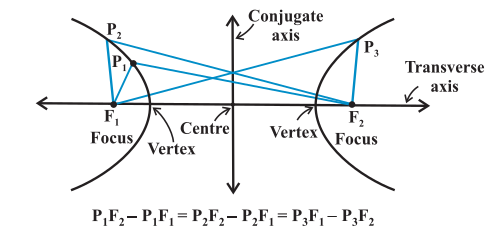
\includegraphics[scale=0.5]{f4.png}
\end{center}
\begin{itemize}
    \item The two fixed points are called the
    \textbf{foci} of the hyperbola
    \item The mid-point of the line segment joining the foci is called the
    \textbf{centre} of the hyperbola
    \item The line through the foci is called the \textbf{transverse axis} and
    the line through the centre and perpendicular to the transverse axis is called the \textbf{conjugate
    axis.}
    \item The points at which the hyperbola
    intersects the transverse axis are called the
    \textbf{vertices} of the hyperbola
    \begin{center}
        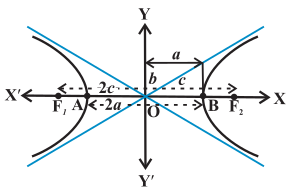
\includegraphics[scale=0.7]{f5.png}
    \end{center}
    \item We denote the distance between the
    two foci by 2c, the distance between two
    vertices (the length of the transverse axis)
    by 2a and we define the quantity b as
   $ b =\sqrt{
    c^2 - a^2}$
\end{itemize}
\subsubsection*{Standard equation of Hyperbola}

\begin{enumerate}
    \item $\frac{x^{2}}{a^{2}}-\frac{y^{2}}{b^{2}}=1$ \begin{center}
        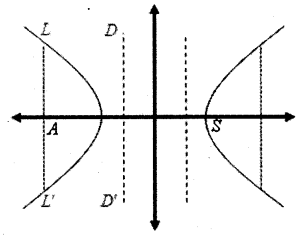
\includegraphics[scale=0.8]{7.png}
    \end{center}
    \begin{itemize}

        \item Focii, S(ae, 0) and S'(-ae, 0) or S(c, 0), S'(-c, 0)
        \item Centre (0, 0)
        \item Vertices A(a, 0) and A'(-a, 0)
        \item Equation of directrix (DD’) is $x = \frac{a}{e}$ and $x = \frac{-a}{e}$
    \end{itemize}
    \item $\frac{y^{2}}{a^{2}}-\frac{x^{2}}{b^{2}}=1$ \begin{center}
        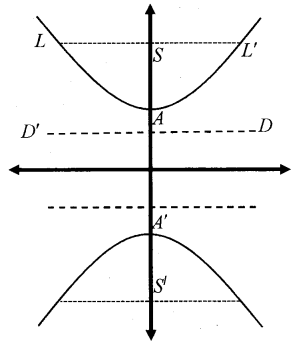
\includegraphics[scale =0.7]{8.png}
    \end{center}
    \begin{itemize}
        \item Eccentricity, $e = \frac{\sqrt{a^2+b^2}}{a}$
        \item Length of Latus rectum (LL’) = $\frac{2b^2}{a}$
        \item Focii, S(0, ae) and S'(0, -ae) or S(0, c), S'(0, -c)
        \item Centre (0, 0)
        \item Vertices A(0, a) anti A'(0, -a)
        \item Equation of directrix (DD’) is $y =\frac{a}{e}$  and $y = \frac{-a}{e}$
    \end{itemize}

\end{enumerate}
\end{multicols}

\end{document}